\RequirePackage{silence}
\documentclass[10pt, compress,british,xcolor={svgnames,dvipsnames,x11names},trans]{beamer}

\usepackage[english]{babel}
\usepackage[utf8]{inputenc}
\usepackage{csquotes}
\usepackage{comment}
\usepackage{tikzsymbols}

\def\area#1{{\color{darkgreen}area:\it #1}}
\def\food#1#2{{Dial. state #1: \color{blue}food:\it #2}}
\def\pricerange#1{{\color{orange}pricerange:\it #1}}
\def\sys#1{{\color{purple}System: \it #1}}
\def\usr#1{{\color{brown}User: \it #1}}
\def\api#1{{\color{blue}DB annotations: \it #1}}

% OP - Ondrej Platek inline 
\definecolor{purple}{RGB}{200,0,200}
\def\OP#1{{\color{purple}OP: \it #1}}
\def\OPdel#1{\bgroup\markoverwith{\textcolor{purple}{\rule[0.5ex]{2pt}{1pt}}}\ULon{#1}}


%%% mtheme customisations
% \usetheme[frametitleformat=regular,progressbar=frametitle,block=fill]{m}
\usetheme[progressbar=frametitle]{m}
\AtBeginSubsection{
\metroset{color/background=dark}
\frame[plain,c]{
  \begin{center}
  \begin{minipage}{25em}
    \usebeamercolor[fg]{section title}
    \usebeamerfont{section title}
    \insertsubsection\\[-1ex]
    \usebeamertemplate*{progress bar in section page}
  \end{minipage}
  \end{center}
}
\metroset{color/background=light}
}
%%%%% end mtheme

\setbeamertemplate{frametitle continuation}[from second]
\setbeamertemplate{bibliography item}[book]

\usetikzlibrary{arrows}
\usetikzlibrary{chains}
\usepackage{tikz-qtree}
\usepackage{multicol}


\usepackage{expex}
%\lingset{glhangindent=2em,glspace=1em,aboveexskip=0pt,belowexskip=0pt,aboveglftskip=-3pt,extraglskip=3pt} %v0.1
%\lingset{exskip=0pt,interpartskip=-3pt,belowpreambleskip=-3pt,belowglpreambleskip=-3pt,aboveglftskip=-3pt,extraglskip=3pt,glhangstyle=none}
\usepackage{relsize}
\usepackage{booktabs,tabularx}
%\usepackage{textcomp}
\usepackage{listings}
\lstset{basicstyle=\ttfamily,breaklines=true,breakatwhitespace=true,
keywordstyle={\color{NavyBlue}\bfseries}, showstringspaces=false,
commentstyle={\color{PaleVioletRed4}},
emphstyle={\color{OliveGreen}\bfseries}
}

\usepackage{algorithmic}
\renewcommand{\algorithmiccomment}[1]{\alert{/* #1 */}}

\usetikzlibrary{shapes.multipart}
\usetikzlibrary{positioning}
\usetikzlibrary{arrows.meta}

\makeatletter
\pgfarrowsdeclare{crow's foot}{crow's foot}
{
  \pgfarrowsleftextend{+-.5\pgflinewidth}%
  \pgfarrowsrightextend{+.5\pgflinewidth}%
}
{
  \pgfutil@tempdima=0.5pt%
  \advance\pgfutil@tempdima by.25\pgflinewidth%
  \pgfsetdash{}{+0pt}%
  \pgfsetmiterjoin%
  \pgfpathmoveto{\pgfqpoint{0pt}{-6\pgfutil@tempdima}}%
  \pgfpathlineto{\pgfqpoint{-6\pgfutil@tempdima}{0pt}}%
  \pgfpathlineto{\pgfqpoint{0pt}{6\pgfutil@tempdima}}%
  \pgfusepathqstroke%
}

\usepackage[os=win]{menukeys}
\usepackage{notoccite}
\usepackage[numbers,sort&compress]{natbib}


\title{{A Dataset of Operator-client Dialogues Aligned with Database Queries for End-to-end Training}}


\author{Ondřej Plátek \& Filip Jurčíček \\ \footnotesize{\texttt{\{oplatek,jurcicek\}@ufal.mff.cuni.cz}}}
\institute{
Institute of Formal and Applied Linguistics\\
Faculty of Mathematics and Physics\\
Charles University in Prague
}

\begin{document}

\maketitle

\begin{frame}\frametitle{Intended scenario}
    \begin{itemize}
        \item DSTC2~\cite{henderson2014dstc2} restaurant domain
        \item User's goal: {\it Chinese} restaurant in {\it a city center}
    \end{itemize}
    \vfill
    \sys{Hello, welcome to the Cambridge restaurant system! \dots } \\
    \usr{I would like a Chinese restaurant} \\
    \sys{A golden house is a Chinese restaurant in the city center} \\
    \dots

\end{frame}


\begin{frame}{Table of contents}
  \setbeamertemplate{section in toc}[sections numbered]
  \tableofcontents[hideallsubsections]
\end{frame}


\section{Motivation}

\begin{frame}\frametitle{Collection scenario}
    {\bf User's goal: {\it Chinese} restaurant in {\it a city center}} \\
    {\ Operator can search a table with restaurant information}
    \vfill
    \usr{I would like a Chinese restaurant} \\
    \api{select restaurant.name food="Chinese"} \\
    \sys{A golden house is a Chinese restaurant in the city center}
\end{frame}

\begin{frame}\frametitle{Why new dataset?}
    \begin{enumerate}
        \item <1> New annotation type
        \item <2> More data
        \item <3> Introduce different level of complexity
        \item <4> Understating the dataset
    \end{enumerate}
\end{frame}

\begin{frame}\frametitle{Annotations for task oriented systems}
    \begin{columns}
        \begin{column}{0.40\textwidth}
            
\includegraphics[width=0.80\textwidth]{is_it_ontology.png}
        \end{column}
        \begin{column}{0.60\textwidth}
            \vfill
            % Todo insert arrow
            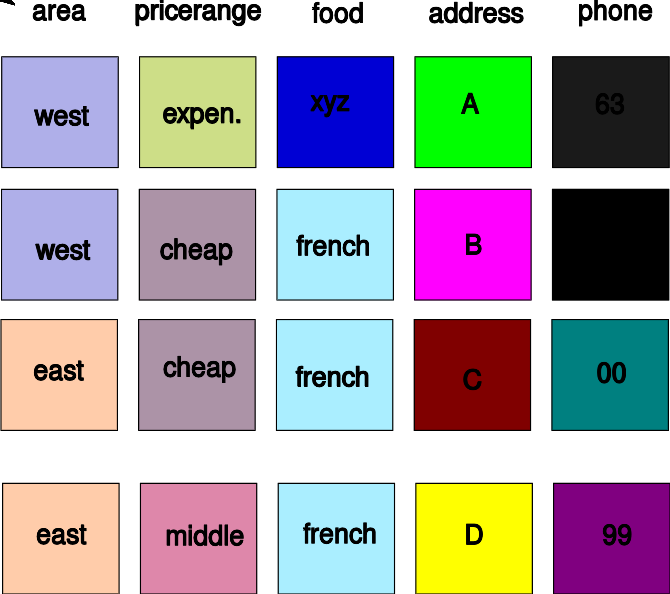
\includegraphics[width=0.90\textwidth]{db_columns.png}
        \end{column}
    \end{columns}
\end{frame}

\begin{frame}\frametitle{Similar to DSTC2\cite{henderson2014dstc2}}
    \begin{enumerate}
        \item Focused on semantics (valid answers) not NLG
        \item Simplified --- single (current) goal, guided via interface  
        \item Different collection scheme --- automatic validation
    \end{enumerate}
\end{frame}


\section{Collection process}

\begin{frame}\frametitle{Offline collection scheme}
    \begin{itemize}
        \item Easy to crowdsource
        \item Easy to check 
        \item Time for annotations\cite{wen2016network}
    \end{itemize}
\end{frame}

\begin{frame}\frametitle{Client interface}
    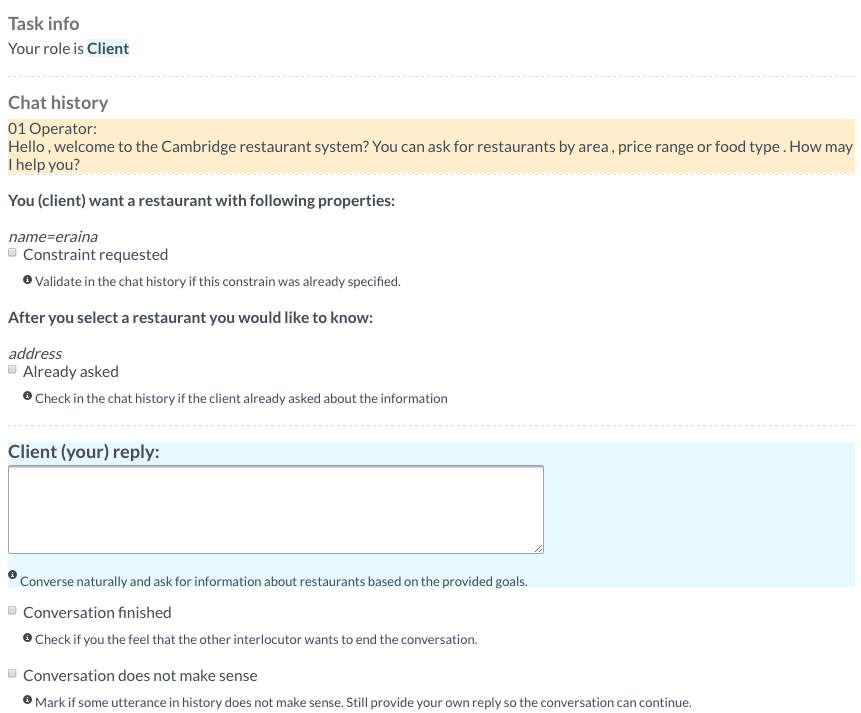
\includegraphics[width=0.90\textwidth]{./gui-annotators-client.png}
\end{frame}

\begin{frame}\frametitle{System interface}
    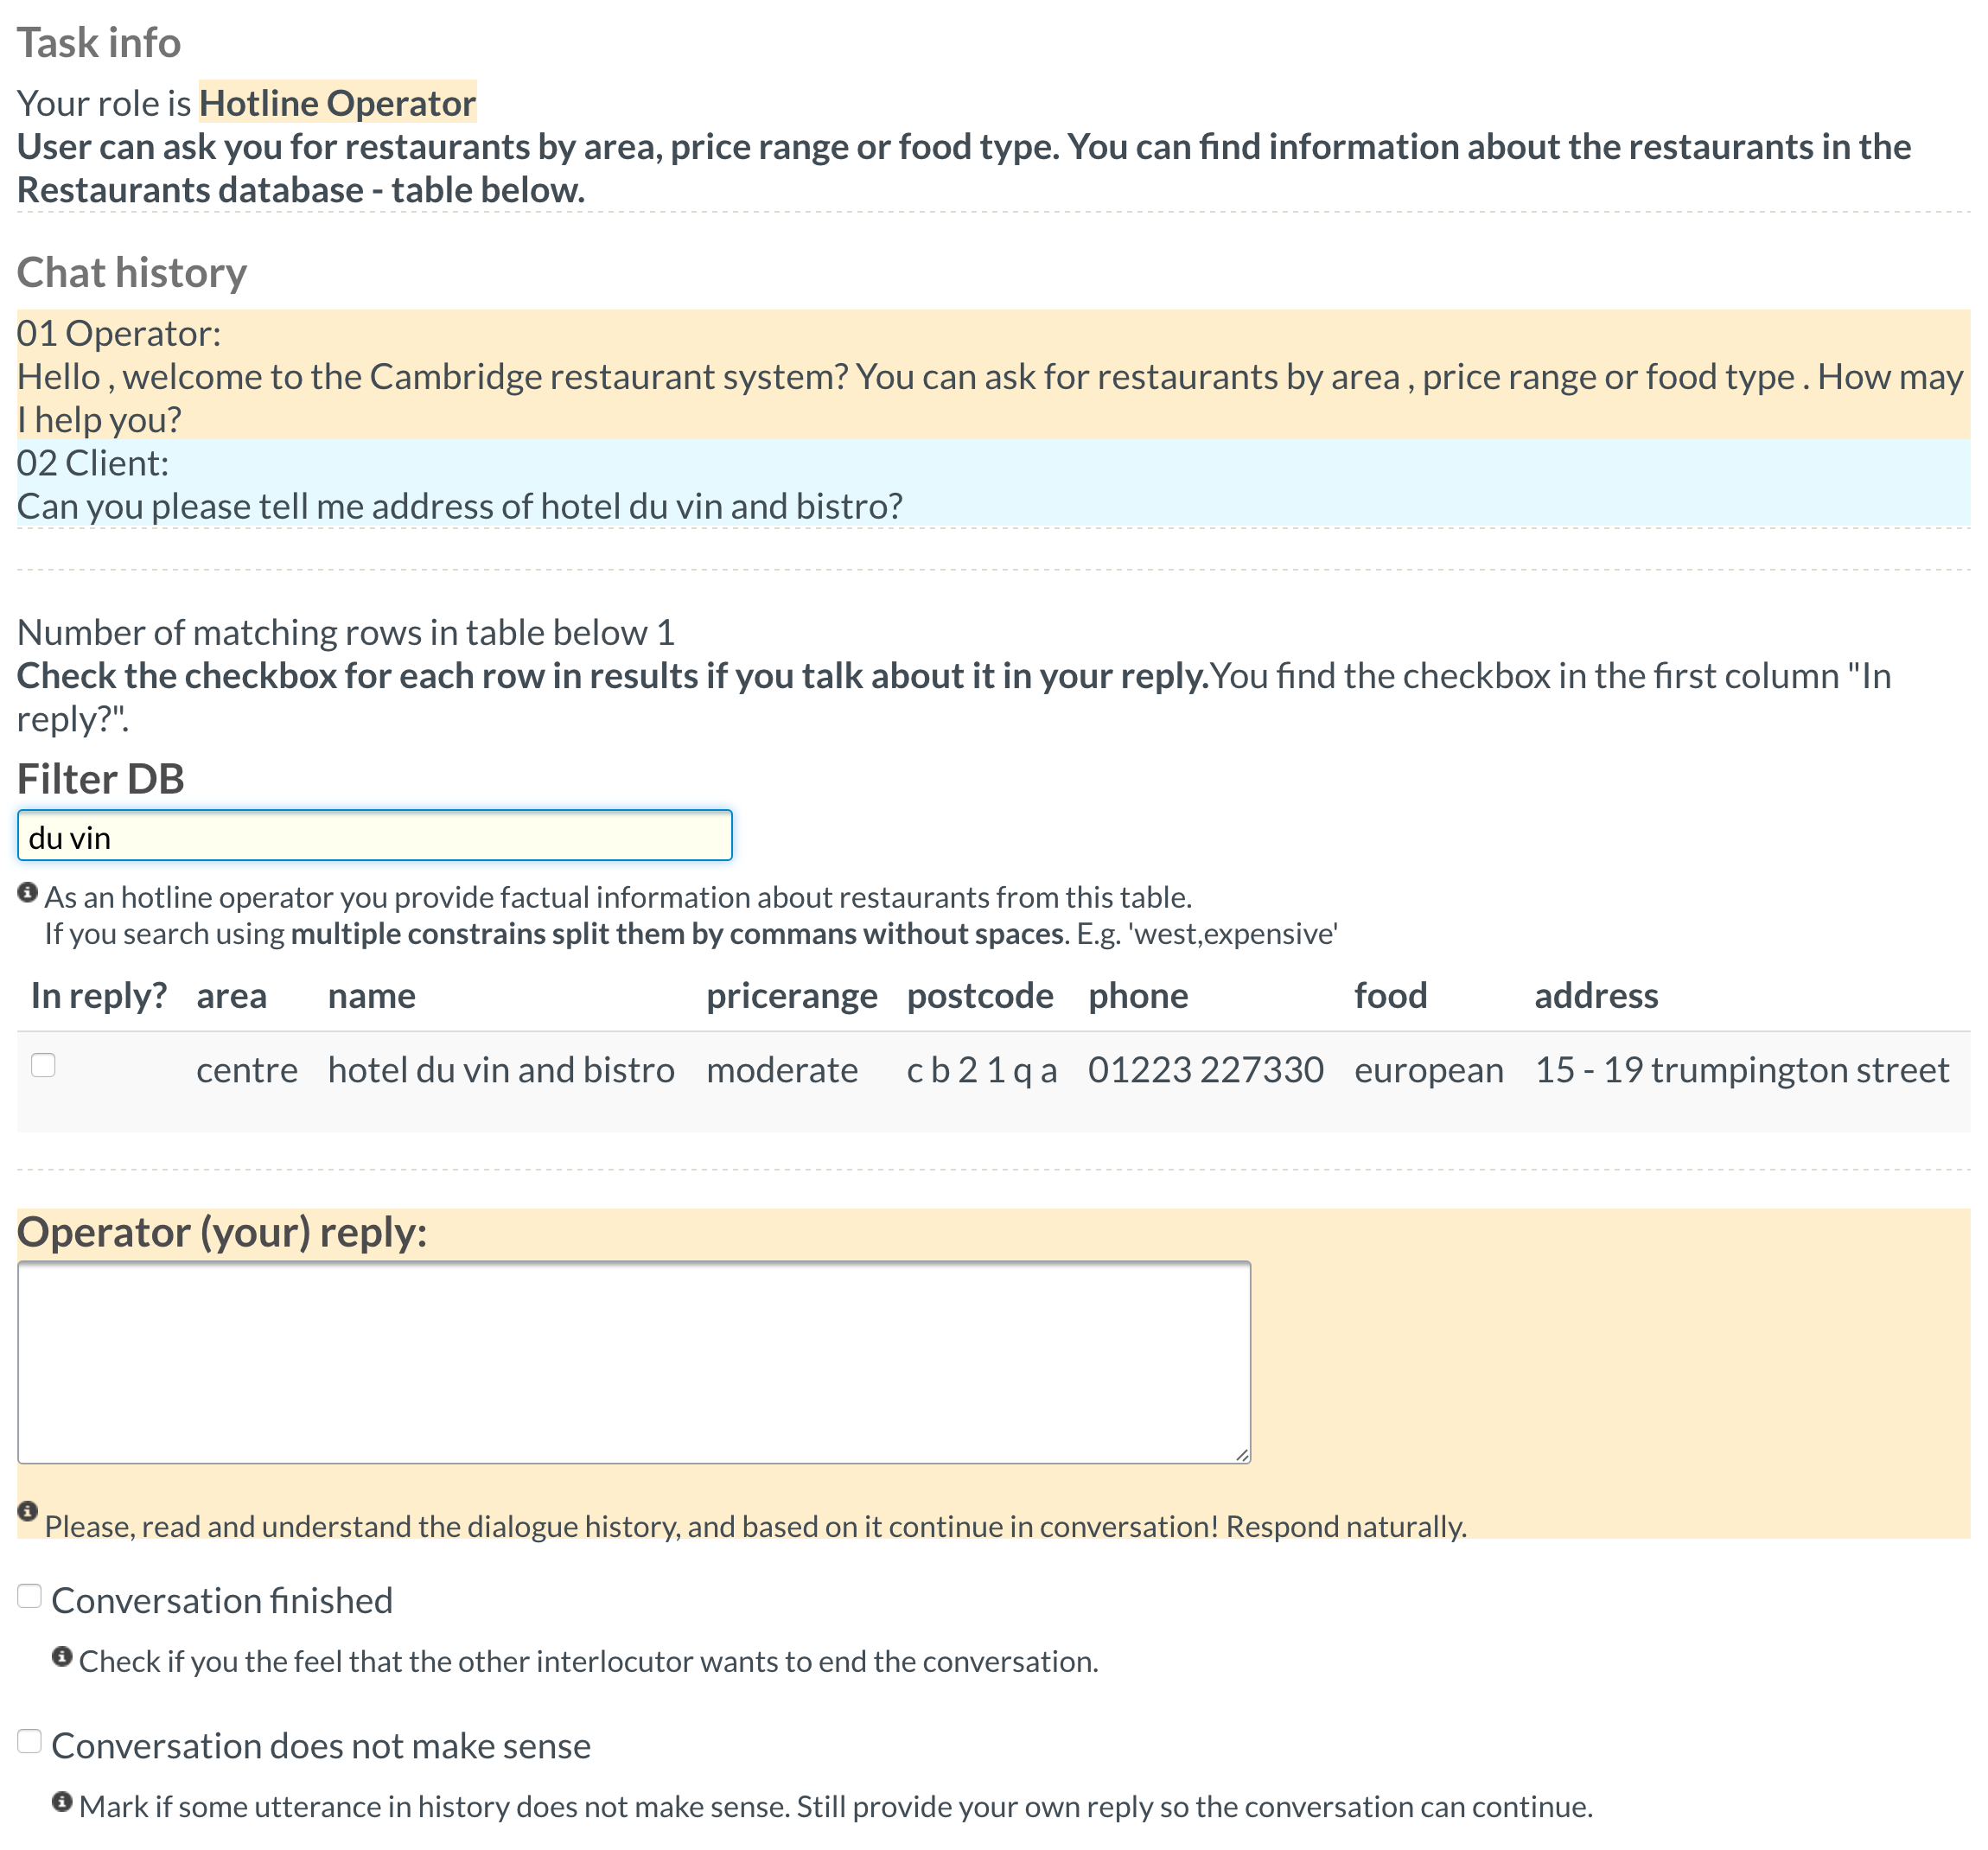
\includegraphics[width=0.90\textwidth]{./gui-annotators-system.png}
\end{frame}

\begin{frame}\frametitle{Collection process}
    \begin{enumerate}
        \item Each job add a single response to each dialogue 
        \item User feedback
        \item Manual control still needed
        \item Goal presented incrementally
    \end{enumerate}
\end{frame}

\section{Dataset sample}

\begin{frame}\frametitle{First finished data}
    \begin{enumerate}
        \item Each job add a single response to each dialogue 
        \item User feedback
        \item Manual control still needed
        \item Goal presented incrementally
    \end{enumerate}
\end{frame}

\begin{frame}\frametitle{First statistics}
    \begin{enumerate}
        \item 62 finished conversations
        \item 3.8 turns (pair of user system replies) collected
        \item User told to ask for 2.4 goals but only 1.9 answered 
        \item 4 correct reports not valid replies
        \item Discarding under \% 35 replies
        \item more than 20\%  
    \end{enumerate}
\end{frame}

\begin{frame}\frametitle{Example}
    \sys{Hello, welcome to the Cambridge restaurant system! \dots } \\
    {\bf User's goal: {\it Chinese restaurant}} \\
    \usr{I would like a Chinese restaurant} \\
    \api{filter: Chinese} \\
    \sys{There is a yu garden} \\
    {\bf User's goal: {\it Chinese restaurant} \& {\it city center}} \\
    \usr{I would like one in the city center} \\
    \api{filter: Chinese, center} \\
    \sys{A golden house is a Chinese restaurant in the city center} \\
    {\bf User's goal: {\it Chinese restaurant} \& {\it city center}} \\
    \usr{cool bye!} \\
    \sys{Glad to help you}
    \dots
\end{frame}

\section{Future work}

\begin{frame}\frametitle{In progress}
    \begin{enumerate}
        \item Apologies for not publishing the dataset!
        \item Detecting end of dialogue automatically
        \item Discourage one shot queries
        \item Automatic validation
    \end{enumerate}
\end{frame}

\begin{frame}\frametitle{Future work}
    \begin{enumerate}
        \item Evaluating usefulness of DB calls in for selecting response 
        \item Pairing crowd-source workers in real-time
        \item Compare real-time and offline annotation scheme
    \end{enumerate}
\end{frame}

\appendix

\begin{frame} \frametitle{Early experiment: Encoder-Decoder with DB sophisticated lies}
{\bf input:} {\it anatolia serves turkish food in the moderate price range what is the phone number and address} \\
{\bf decoded:} {\it The phone number of {\bf meghna} is {\bf 01223 727410} . EOS} \\
{\bf target:} {\it The phone number of anatolia is {\bf 01223 362372} and it is on 30 Bridge Street City Centre . EOS}
\end{frame}

\begin{frame}[allowframebreaks]
        \frametitle{References}
        \bibliographystyle{unsrtnat}
        \bibliography{literature.bib}
\end{frame}



\end{document}
